\documentclass[12pt, a4paper]{article}
\usepackage[utf8]{inputenc}
%\usepackage[IL2]{fontenc}
\usepackage[czech]{babel}
\usepackage[pdftex]{graphicx}
\usepackage{mathtools}
\usepackage{amsmath}
\usepackage{svg}
\usepackage{textcomp}
\usepackage{listings,xcolor}
\usepackage[final]{pdfpages}
\usepackage{verbatim}
\usepackage{todonotes}
\usepackage[T1]{fontenc}
\usepackage{multirow}

\usepackage[nottoc,notlot,notlof]{tocbibind}
\usepackage[pdftex,hypertexnames=false]{hyperref}
\hypersetup{colorlinks=true,
  unicode=true,
  linkcolor=black,
  citecolor=black,
  urlcolor=black,
  bookmarksopen=true}

\newcommand{\floor}[1]{\lfloor #1 \rfloor}

\title{\textbf{Dokumentace semestrální práce} \\KIV/PPR}
\author{Vojtěch Danišík}
\begin{document}

\begin{titlepage} 
	\newcommand{\HRule}{\rule{\linewidth}{0.5mm}} 
	\begin{center}
	
\includegraphics[width=12cm]{img/fav_logo}\\
	\end{center}
	\textsc{\LARGE Západočeská univerzita v Plzni}\\[1.5cm] 	
	\textsc{\Large Paralelní programování}\\[0.5cm] 
	\textsc{\large KIV/PPR2}\\[0.5cm] 
	\HRule\\[0.4cm]
	{\huge\bfseries Dokumentace semestrální práce}\\[0.4cm] 
	\HRule\\[1.5cm]

	\begin{minipage}{0.4\textwidth}
		\begin{flushleft}
			\large
			Vojtěch \textsc{Danišík}\newline
			A19N0028P\newline
			danisik@students.zcu.cz
		\end{flushleft}
	\end{minipage}
	\vfill\vfill\vfill
	\begin{flushright}
	{\large\today}
	\end{flushright}
	\vfill 
\end{titlepage}
\newpage
\tableofcontents
\newpage

\section{Zadání}
Program semestrální práce dostane, jako jeden z parametrů, zadaný souboru, přístupný pouze pro čtení. Bude ho interpretovat jako čísla v plovoucí čárce - 64-bitový double. Program najde číslo na arbitrárně zadaném percentilu, další z parametrů, a vypíše první a poslední pozici v souboru, na které se toto číslo nachází.\\

\noindent Program se bude spouštět následovně: \\

\noindent pprsolver.exe soubor percentil procesor
\begin{itemize}
\item soubor - cesta k souboru, může být relativní k program.exe, ale i absolutní
\item percentil - číslo 1 - 100
\item procesor - řetězec určujíící, na jakém procesoru a jak výpočet proběhne
\begin{itemize}
\item single - jednovláknový výpočet na CPU
\item SMP - vícevláknový výpočet na CPU
\item anebo název OpenCL zařízení kompatibilní GPGPU - pozor, v systému může být několik OpenCL platforem
\end{itemize}
\item Součástí programu bude watchdog vlákno, které bude hlídat správnou funkci programu
\end{itemize}
Testovaný soubor bude velký několik GB, ale paměť bude omezená na 250 MB. Zařídí validátor. Program musí skončit do 15 minut na iCore7 Skylake. \\
\\
\noindent Explicitní upozornění dle postupných dotazů z řad studentů:
\begin{itemize}
\item Program nebude mít povoleno vytvářet soubory na disku.
\item Jako čísla budete uvažovat pouze ty 8-bytové sekvence, pro které std::fpclassify vrátí FP\_NORMAL nebo FP\_ZERO. Jiné sekvence budete ignorovat. Všechny nuly jsou si stejně rovné.
\item Pozice v souboru vypisujte v bytech, tj. indexováno od nuly.
\item Hexadecimální číslo vypište např. pomocí std::hexfloat.
\end{itemize}

\newpage







\section{Analýza}
\subsection{Čísla s plovoucí čárkou}
Čísla s plovoucí čárkou jsou taková čísla, která jsou moc malá nebo velká pro vyjádření v pevné řádové čárce. Čísla jsou obecně uložena jako určité množství platných číslic vynásobený exponentem. Základem exponentu bývá většinou 2, 10 nebo 16. \\
\indent V případě, že bychom chtěli pomocí těchto čísel vyjadřovat intervaly bucketů v histogramu, tak je potřeba počítat s velikou časovou režií při zpracování dat. Pro všechna načtená čísla s plovoucí čárkou je potřeba zjistit do jakého bucketu bude patřit, což lze zjistit pomocí vyhledávacích algoritmů. Nejrychlejší dostupný vyhledávací algoritmus je pro nás \textit{binární vyhledávání}, které má časovou složitost \textit{O(log n)}.
\indent Rychlejší řešení je reprezentace hodnot jako celočíselných indexů za pomoci \textit{type punningu}. Type punning je programovací technika, pomocí které lze měnit datový typ proměnné, aniž bychom jakkoliv změnili její hodnotu (v bitové reprezentaci). Tímto řešením by odpadla potřeba pro každou hodnotu s plovoucí čárkou využívat binární vyhledávání, které je pro tak velké množství čísel relativně pomalé.

\subsection{Symetrický multiprocesor}
Symetrický multiprocesor (SMP) je označení pro druh víceprocesorových systémů, kde jsou dva nebo více procesorů připojeny k jedné sdílené hlavní paměti, mají plný přístup ke všem vstupním a výstupním zařízením a jsou řízeny jedinou instancí operačního systému. \\
\indent Operační systém zachází se všemi procesory stejně, žádný si nevyhrazuje pro speciální účely. \\
\indent Každý procesor je propojen s vlastní vyrovnávací pamětí, která může být rozdělena na vyrovnávací paměť určenou pro data a vyrovnávací paměť pro instrukce). Tato vyrovnávací paměť je napojena na interní sběrnici, která zajišťuje řízení přenosu dat mezi těmito paměťmi a pamětí operačního systému (viz obrázek č. \ref{fig:smp}).\\
\indent V této úloze bude SMP sloužit hlavně pro paralelní zpracování vstupního souboru, kdy hlavní vlákno může (skoro) bez omezení stále načítat datové bloky a vedlejší vlákna budou mezitím zpracovávat načtené bloky dat. V případě velmi rychlého zpracovávání dat bude nutné odladit počet vláken tak, aby nedocházelo ke zbytečnému uspávání jak vedlejších vláken, tak i hlavního vlákna.


\begin{figure}[!h]
\centering
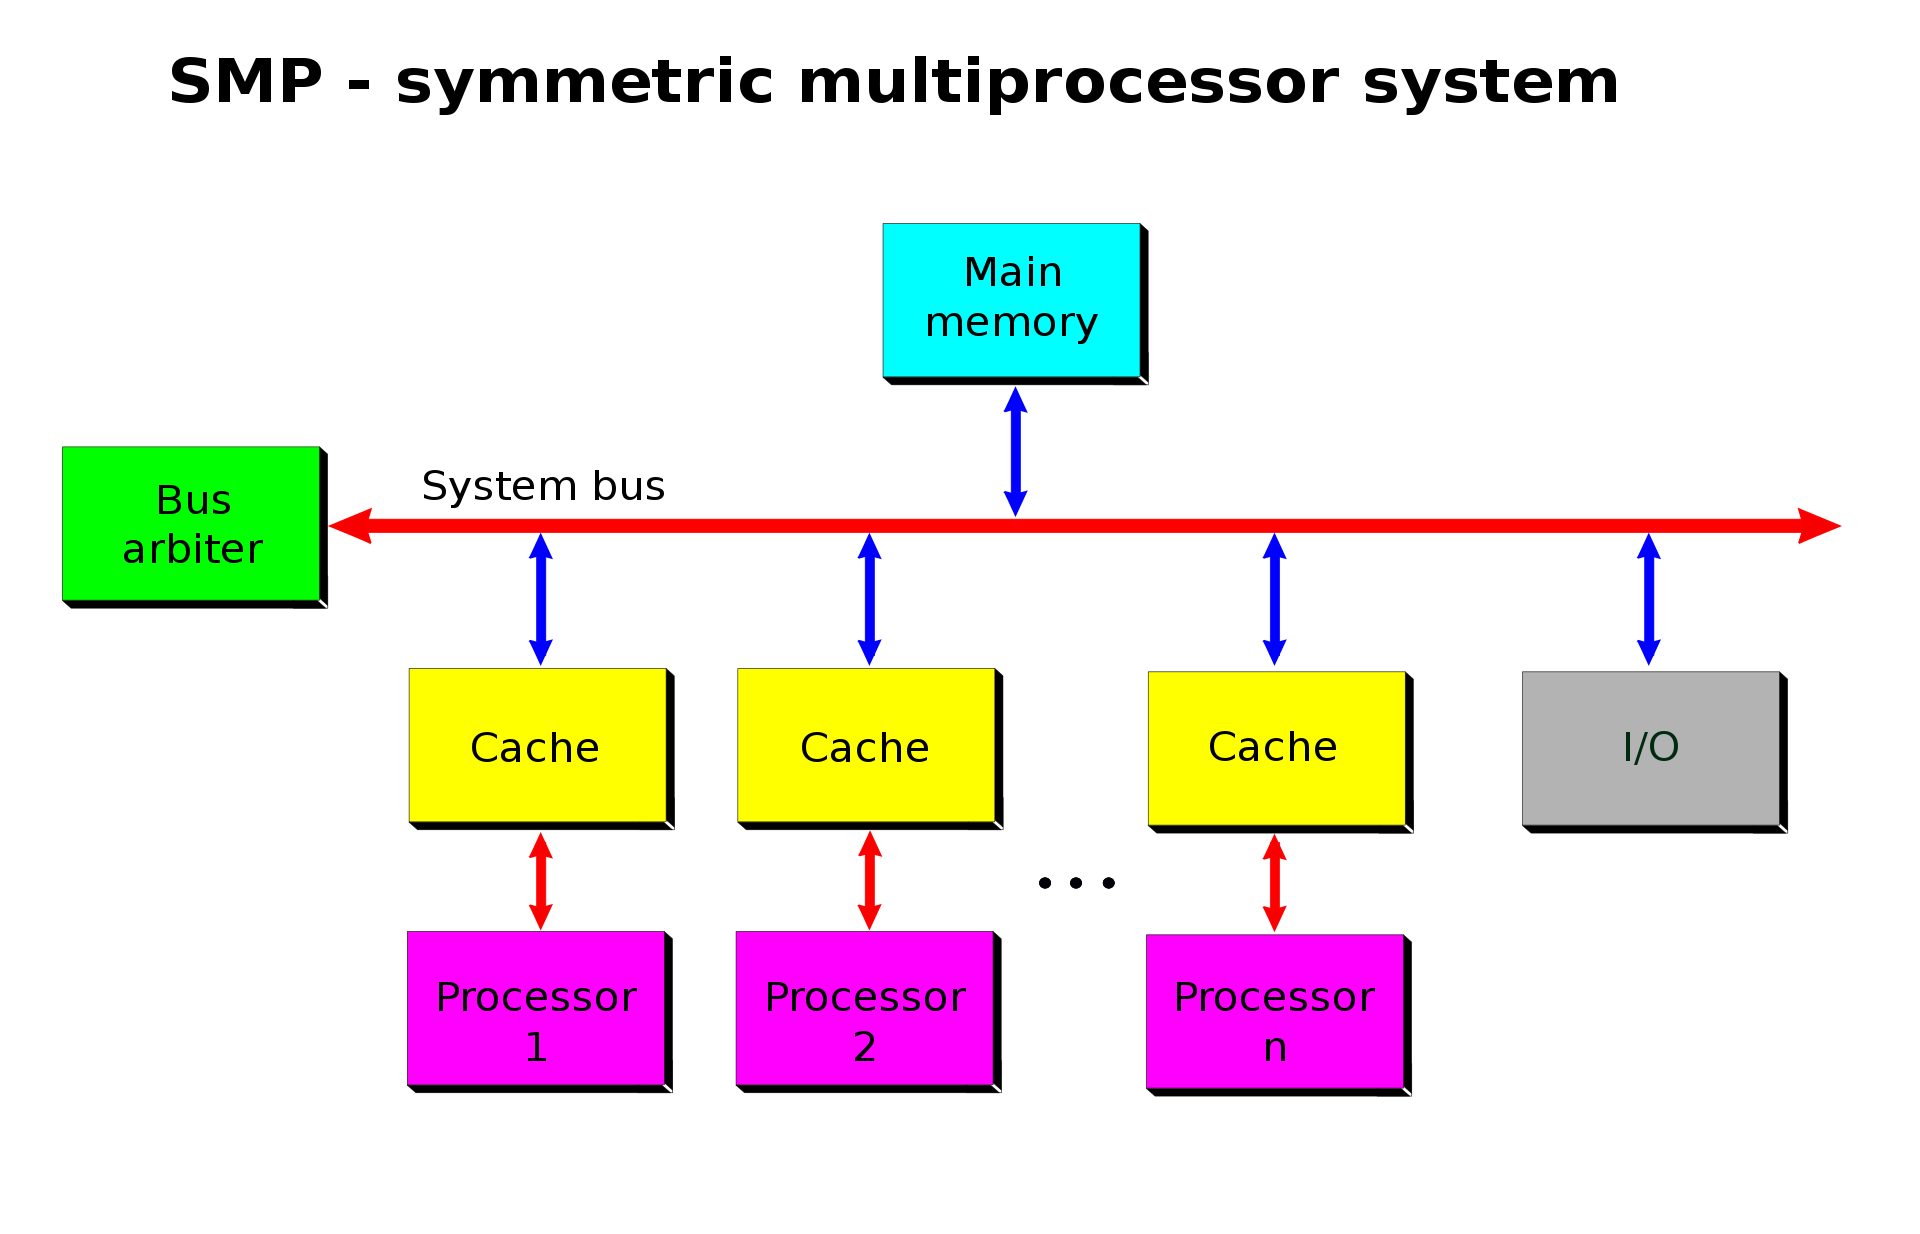
\includegraphics[width=14cm]{img/smp}
\caption{Ukázka SMP}
\label{fig:smp}
\end{figure}

\subsection{GPGPU}
\textbf{General-purpose computing on graphics processing units} (neboli GPGPU) je způsob využití paralelizace na grafické kartě k výpočtům, které jsou jinak zpracovány pomocí \textit{Central processing unit} (CPU).\\
\indent Pomocí GPGPU pipeline lze paralelizovat proces mezi jedním až více GPU a CPU. Protože GPU operuje na nižších frekvencích, tak grafické karty mají o to více procesorů, díky čemuž lze zpracovávat více dat za sekundu. \\
\indent V této úloze bude GPGPU sloužit pro zpracování bloků dat - klasifikace a rozřazení do jednotlivých bucketů. Každému vláknu lze předat část dat (ideálně vždy jedno číslo), které klasifikuje a zjištěnému bucketu přičte frekvenci.Tento přístup by zaručoval rychlejší zpracování celého souboru.\\

\newpage







\section{Implementace}
V implementaci jsou popsány dva postupy řešení - původní, který nesplňoval časový limit pro single procesor, a nový, který je více časově efektivnější.

\subsection{Původní řešení}
Původní řešení zahrnovalo práce s čísly v plovoucí čárce - minima a maxima histogramu / bucketů, binární vyhledávání.

\subsubsection{Inicializace bucketů}
Inicializace bucketů a jejich minimálních a maximálních povolených hodnot se provádělo pomocí vzorce č. \ref{eq:step_calculation}:
\begin{equation}
step = |\frac{min}{bucket\_count}| + \frac{max}{bucket\_count} \\
\label{eq:step_calculation} 
\end{equation}
kde \textit{step} je krok pro spočítání maximální povolené hodnoty bucketu, \textit{min} a \textit{max} jsou minimální a maximální povolené hodnoty v histogramu, \textit{bucket\_count} je počet bucketů v histogramu.

Buckety jsou seřazeny vzestupně (první bucket má minimální hodnotu rovno minimální hodnotě histogramu, poslední bucket má maximální hodnotu rovno maximální hodnotě histogramu).

\subsubsection{Zpracování dat} \label{sssec:old_zpracovani}
Pro každou iteraci zpracování se prováděly tyto kroky:
\begin{enumerate}
\item Načtení datového bloku o velikosti 1 MB.
\item Kontrola validity všech načtených double čísel v datovém bloku - kontrola pomocí metody std::fpclassify.
\item Rozřazení čísel do správných bucketů pomocí binárního vyhledávání.
\begin{itemize}
\item Rozřazování probíhalo na základě porovnání načteného čísla s minimem a maximem daného bucketu.
\item Binární vyhledávání bylo řešeno rekurzivně.
\item Při rozřazování se také aktualizovala minimální a maximální načtená hodnota v daném bucketu.
\end{itemize}
\item Inkrementace čítačů načtených hodnot.
\begin{itemize}
\item Čítač všech načtených validních hodnot.
\item Čítač pro hodnoty, které jsou validní, ale menší jak definovaná minimální hodnota histogramu.
\end{itemize}
\item Nalezení bucketu pomocí percentilu (viz sekce č. \ref{ssec:bucket_find}).
\end{enumerate}

\subsubsection{Kontrola nalezeného bucketu}
Po zpracování dat a nalezení bucketu bylo potřeba zkontrolovat, zda bucket je reprezentován jako číslo nebo jako interval. \\
\indent V případě, že nalezená minimální a maximální hodnota ze souboru v daném bucketu jsou stejná, pak stačí pro nalezené číslo najít jeho pozici (viz sekce \ref{ssec:position}) v souboru a program se ukončí. \\
\indent V případě, že nalezená minimální a maximální hodnota ze souboru v daném bucketu nejsou stejná, pak je potřeba nastavit nové minimum a maximum histogramu a opakovat celý proces zpracování dat znova.

\subsection{Nové řešení}
Nové řešení zahrnuje práce s celými čísly (indexy), převodem hodnot s plovoucí čárkou na celá čísla, kódování záporných čísel do sign-magnitude formátu a obcházení datových typů.\\
\indent Control flow diagram lze vidět na obrázku č. \ref{fig:controlflow}. Data flow diagram lze vidět na obrázku č. \ref{fig:dataflow}.

\subsubsection{Inicializace histogramu}
Při inicializaci histogramu bylo potřeba provést několik věcí. Jako první se vytvoří buckety s nastavenou frekvencí na hodnotu 0 a přiřadí se jim index. Následně bylo potřeba spočítat velikost jednoho bucketu (viz vzorec č. \ref{eq:size}).
\begin{equation}
bucket\_size =  \frac{max - min}{bucket\_count - 1} + x; x = 
\begin{cases}
1	&	(max - min) \% (bucket\_count - 1) > 0	\\
0	& 	(max - min) \% (bucket\_count - 1) = 0
\end{cases} \\
\label{eq:size} 
\end{equation}
kde \textit{bucket\_size} je velikost bucketu, \textit{max} je maximální hodnota histogramu, \textit{min} je minimální hodnota histogramu a \textit{bucket\_count} je počet bucketů v histogramu.\\

\noindent Následně se bylo potřeba vypočítat offset pro bucket indexy (viz vzorec č. \ref{eq:offset}).
\begin{equation}
bucket\_index\_offset = \frac{-min}{bucket\_size}  \\
\label{eq:offset} 
\end{equation}
kde \textit{bucket\_index\_offset} je offset pro index bucketu, \textit{min} je minimální hodnota histogramu a \textit{bucket\_size} je vypočítaná velikost bucketu. \\


\noindent Velikost bucketu a offset pro index bucketu se budou používat při převodu hodnoty na index (a zpět).

\subsubsection{Zpracování dat} \label{sssec:new_zpracovani}
Rozdíl ve zpracování dat oproti starému řešení spočíval v převádění hodnot s plovoucí čárkou na celočíselné indexy, což je o mnoho rychlejší jak binární vyhledávání. \\
Převod je realizován ve dvou krocích:
\begin{enumerate}
\item Uložení hodnoty s plovoucí čárkou do binární podoby.
\item Převedení hodnoty v binární podobě ze sign-magnitude formátu.\\
\end{enumerate}

\noindent Po převodu hodnoty lze vypočítat index bucketu, do kterého dané číslo patří. Výpočet indexu lze vidět na vzorci č. \ref{eq:valueindex}.
\begin{equation}
index = \frac{value}{bucket\_size} + bucket\_index\_offset  \\
\label{eq:valueindex} 
\end{equation}


\subsubsection{Kontrola nalezeného bucketu}
Kontrola nalezeného bucketu u nového řešení byla jednodušší, protože se kontrolovala pouze velikost nalezeného bucketu. \\
\indent Pokud velikost bucketu byla rovna jedné, tak se pouze index bucketu převedl zpět na číslo s plovoucí čárkou.\\
\indent Pokud velikost bucketu byla větší jak jedna, jednalo se o interval. Index nalezeného bucketu se převedl zpět ze sign-magnitude formátu a byl určen jako minimální hodnota histogramu. Maximální hodnota histogramu byla určena jako součet minima a velikosti bucketu a celý postup se opakoval.

\newpage
\subsubsection{Control flow diagram}
\begin{figure}[!h]
\centering
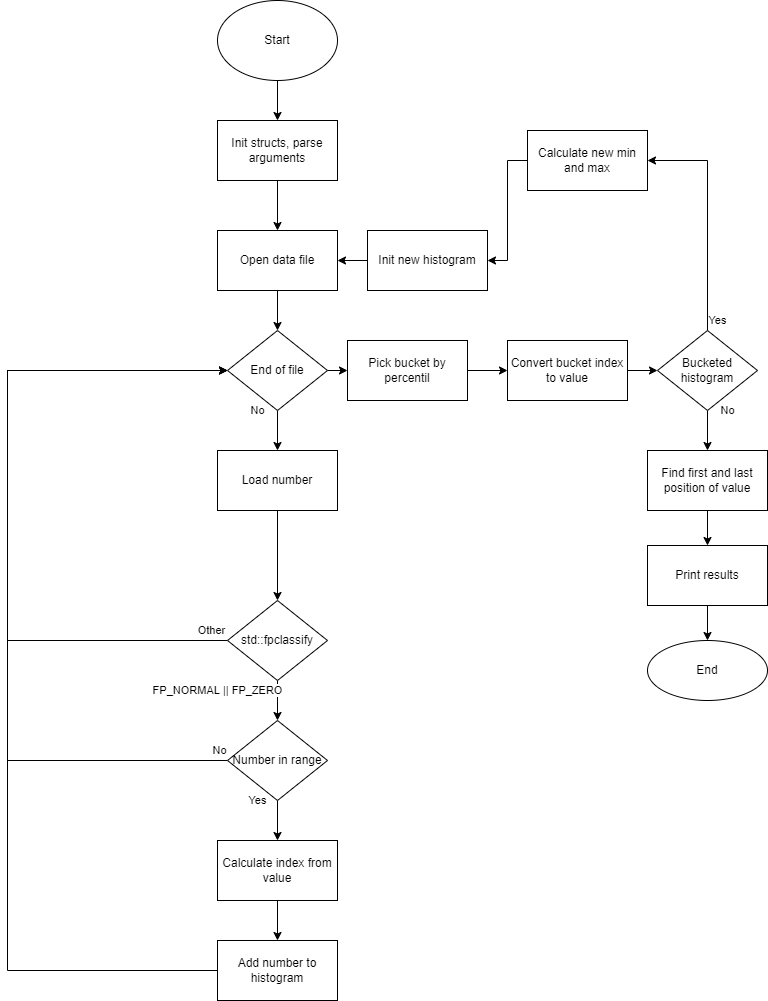
\includegraphics[width=14cm]{img/control_flow}
\caption{Control-flow diagram}
\label{fig:controlflow}
\end{figure}
\newpage

\subsubsection{Data flow diagram}
\begin{figure}[!h]
\centering
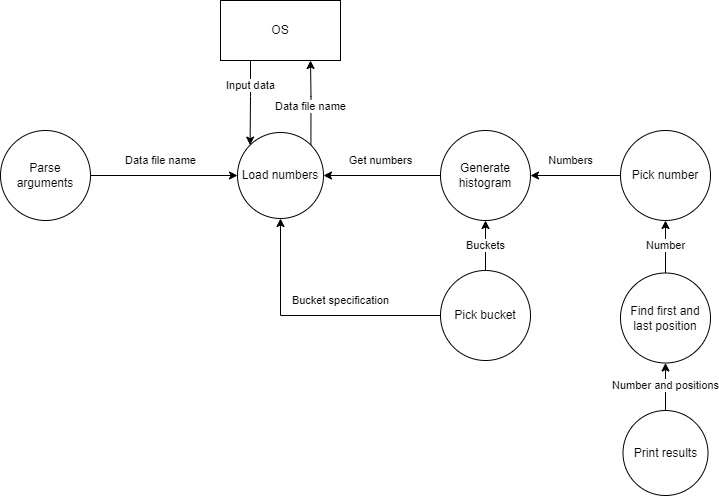
\includegraphics[width=14cm]{img/data_flow}
\caption{Data-flow diagram}
\label{fig:dataflow}
\end{figure}
\newpage

\subsection{Nalezení bucketu pomocí percentilu}\label{ssec:bucket_find}
Po zpracování všech datových bloků v dané iteraci bylo potřeba najít výsledný bucket podle vstupního percentilu. Nejdříve bylo potřeba spočítat pozici čísla pomocí vzorečku č. \ref{eq:percentile_position}:

\begin{equation}
calculated\_position =  \floor{\frac{numbers\_count \cdot percentile}{100}}\\
\label{eq:percentile_position} 
\end{equation}
kde \textit{calculated\_position} je pozice hledaného čísla, \textit{numbers\_count} je počet všech hodnot a \textit{percentile} je vstupní hodnota percentilu (v procentech).\\

\indent Následně se definuje kumulativní frekvence, ke které se přičtě počet hodnot, které jsou menší jak definovaná minimální hodnota histogramu. Po definici kumulativní frekvence se prochází všechny buckety a sčítá se jejich frekvence s kumulativní frekvencí do té doby, dokud kumulativní frekvence je menší nebo rovna vypočtené pozici \textit{calculated\_position}. Jakmile je kumulativní frekvence větší jak spočtená pozice, tak jsme našli náš hledaný bucket na daném percentilu.

\subsection{Nalezení pozice hodnoty v souboru}  \label{ssec:position}
Pro nalezení pozice hodnoty je potřeba postupně načíst celý soubor a porovnávat aktuální první a poslední pozici v souboru. Při inicializaci první pozice je nutné nastavit hodnotu na maximální hodnotu datového typu, zatímco pro poslední pozici je nutné nastavit hodnotu na minimální daného datového typu. Nalezené pozice se následně vynásobí osmi (pozice chceme v bytech).

\subsection{Watchdog}
Watchdog vlákno bylo realizováno jako jedno vlákno, které má v sobě čítač reprezentující počet uběhnutých milisekund, kdy aplikace nevykonává žádnou práci. Resetování čítače se provádí pomocí metody \textit{reset()}, volané skoro ve všech metodách. Limit pro ukončení aplikace je nastaven na 10 sekund neaktivity.

\subsection{Symetrický multiprocesor}
Při použití symetrického mutliprocesoru se vytvoří 10 vláken, které mají za úkol zpracovávat datové bloky viz sekce č. \ref{sssec:old_zpracovani}, \ref{sssec:new_zpracovani}.\\
\indent Předávání dat vláknům je zařízeno pomocí blokovací fronty, jejíž maximální velikost je nastavena na 40 bloků. Blokovací fronta funguje na způsob \textit{single producent - multiple consuments}. \\
\indent Hlavní vlákno (single producent) načítá datové bloky a vkládá je do fronty. V případě, že fronta je zaplněná, se hlavní vlákno uspí pomocí podmínkové proměnné. \\
\indent Vytvořená vlákna (multiple consuments) vybírají z fronty datové bloky a zpracovávají je. V případě, že fronta je prázdná, se vlákno uspí pomocí podmínkové proměnné. \\
\indent Po ukončení zpracování dat v dané iteraci je z vlákna předán zpět jeho histogram, který se následně spojí s hlavním histogramem.










\section{Uživatelská dokumentace}
\noindent Aplikace potřebuje ke správnému spuštění tři povinné argumenty (viz obrázek č.\ref{fig:arguments}):\\

\noindent pprsolver.exe <path\_to\_file> <percentile> <processor>

\begin{itemize}
\item path\_to\_file - relativní / absolutní cesta k souboru s daty
\item percentil - číslo 1 - 100
\item procesor - Typ procesoru, který se má použít pro výpočet:
\begin{itemize}
\item single - jednovláknový výpočet na CPU
\item SMP - vícevláknový výpočet na CPU
\item název OpenCL zařízení - př. NVIDIA GeForce 940MX
\end{itemize}
\end{itemize}

\begin{figure}[h!]
\centering
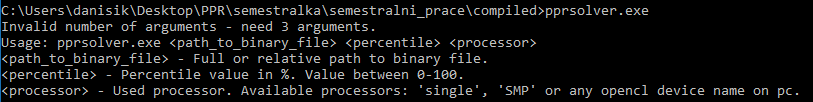
\includegraphics[width=16cm]{img/console_invalid}
\caption{Výstup z konzole - argumenty programu}
\label{fig:arguments}
\end{figure}

\noindent Výstup programu (viz obrázek č.\ref{fig:output}) je ve formátu:\\

\noindent <value\_in\_hex> <first\_position> <last\_position>\\

\noindent Popis hodnot:
\begin{itemize}
\item value\_in\_hex - nalezená hodnota na daném percentilu v hex formátu
\item first\_position - první pozice nalezené hodnoty v souboru v bytech
\item last\_position - poslední pozice nalezené hodnoty v souboru v bytech
\end{itemize}

\begin{figure}[h!]
\centering
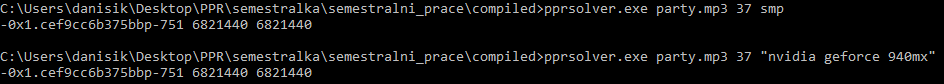
\includegraphics[width=16cm]{img/console_output}
\caption{Výstup z konzole - ukázka použití a výstupu programu}
\label{fig:output}
\end{figure}

\noindent Pozn. Typ procesoru je case-insensitive, což znamená, že pro single procesor lze použít - single, Single, SINGLE, ...

\newpage
\section{Výsledky testování}
Při testování byly použity 2 různě veliké soubory. Rychlost výpočtu pro OpenCL u starého řešení není zmíněna z důvodu změny algoritmu.

\noindent Testovací stroj:
\begin{itemize}
\item CPU: Intel Core i5-8250
\item Grafická karta: NVIDIA GeForce 940MX, Intel UHD Graphics 620
\item Disk: HDD
\item OS: Windows Home 10\\
\end{itemize}

\noindent Soubor: MP3; velikost: 6,8 MB
\begin{table}[h!]
\centering
\begin{tabular}{ |p{3cm}||p{4cm}|p{4cm}|  }
 \hline
 Typ procesoru& Rychlost výpočtu [ s ] (staré řešení)  & Rychlost výpočtu [ s ] (nové řešení)\\
 \hline
 Single   & 1.1    &0.1\\ 
 SMP &   0.4  & 0.2 \\
 NVIDIA &(neimplementováno) & 1.5\\
 Intel  & (neimplementováno)    &2.8\\
 \hline
\end{tabular}
\caption{Porovnání rychlosti výpočtu pro soubor s velikostí 6,8 MB\\\\}
\end{table}

\noindent Soubor: Ubuntu 20.04.3 LTS (iso); velikost: 3 GB
\begin{table}[h!]
\centering
\begin{tabular}{ |p{3cm}||p{4cm}|p{4cm}|  }
 \hline
 Typ procesoru& Rychlost výpočtu [ s ] (staré řešení)  & Rychlost výpočtu [ s ] (nové řešení)\\
 \hline
 Single   & 950    &70\\ 
 SMP &   375  & 65 \\
 NVIDIA &(neimplementováno) & 105\\
 Intel  & (neimplementováno)    &77\\
 \hline
\end{tabular}
\caption{Porovnání rychlosti výpočtu pro soubor s velikostí 3 GB\\}
\end{table}

\noindent Z výsledků lze vidět, že nové řešení je oproti starému řešení mnohonásobně rychlejší. Zároveň lze zmínit rychlost SMP oproti Single CPU, u které se očekávalo mnohem větší zrychlení (nejspíše zapříčiněno neideální implementací vláken / producenta-konzumenta).

\newpage

\section{Závěr}
Výsledný program splňuje všechny požadavky zadání. Program má správně ošetřeny vstupní parametry a výsledkem programu je nalezená hodnota na daném percentilu a její pozice v souboru.\\
\indent Pro soubor o velikosti 3 GB byla rychlost výpočtu v nejhorším případě (OpenCL NVIDIA) zhruba 105 sekund. Paměťová náročnost byla v nejhorším případě (OpenCL) maximálně 160 MB. Při porovnání rychlosti výpočtů starého a nového řešení se podařilo urychlit Single CPU v průměru 10x a SMP v průměru 6x, zatímco paměťová náročnost zůstala neměnná. \\
\indent Z výsledků testování také vyplývá, že rychlost výpočtu SMP oproti single CPU je nepatrně rychlejší, což indikuje špatnou implementaci ať už BlockingQueue (časté čekání vláken na datové bloky), nebo práce s vlákny.
\newpage
	
\end{document}